\documentclass{perassignments}



\usepackage{hyperref}
\usepackage[abjad]{pertheorems}
\usepackage{codestyles}
% \usepackage{english-theorems}
\usepackage{float}
\usepackage{mathtools}
\usepackage{amsmath}
\usepackage{common}
\usepackage{xepersian}



\settextfont[]{XBNiloofar}
\setmathdigitfont{XBTabriz}


\CourseName[آز سیستم دیجیتال]
\Semester[تابستان]
\Year[01]
\Prof[دکتر انصاری]
\Dept[دانشکده مهندسی کامپیوتر]
\CollabFirst[عماد زین‌اوقلی]{98103267}
\CollabSecond[عطا رحیم‌زاده]{98170805}
\CollabThird[سپنتا رحمانی‌زاده]{98110049}

\renewcommand{\maketitle}{\MakeMyLabTitle}
\newcommand{\vars}[1]{\texttt{#1}}
\newcommand{\varseq}[1]{\texttt{#1} \;}
\allowdisplaybreaks


\begin{document}
	\maketitle
	\section{آزمایش چهارم}
	در این آزمایش بایستی یک مدار پشته ۴ بیتی به اندازه ۸ طراحی کنیم.
	 \subsection{مدار اصلی}
	در ماژول 
	\lr{stack}
	پشته‌ای ۴ بیتی به اندازه ۸ طراحی کردیم. در این پشته دو متغیر داریم. متغیر 
	\vars{stack}
	یک آرایه ۸-تایی از ثبات‌های ۴ بیتی است که به عنوان حافظه پشته از آن استفاده می‌شود. متغیر 
	\vars{hotbit\_address}
	یک ثبات ۹ بیتی است که اولین خانه خالی پشته اشاره می‌کند. بدین ترتیب، زمانی که مقدار آن
	\(9'b0\_0000\_0001\)
	است، پشته خالی است و زمانی که مقدار آن برابر با 
	\(9'b1\_0000\_0000\)
	است پشته پر است. سیگنال 
	\vars{resN}
	به صورت 
	\lr{synchronous}
	عمل می‌کند به مقادیر درون 
	\vars{stack}
	صفر می‌کند و 
	\vars{hotbit\_address}
	را برابر با 
	\(9'b0\_0000\_0001\)
	قرار می‌دهد. اگر سیگنال 
	\vars{push}
	فعال باشد و پشته پر نباشد (سیگنال 
	\vars{full}
	غیر فعال باشد) آنگاه مقدار ورودی 
	\vars{data\_in}
	درون پشته می‌ریزیم و مقدار 
	\vars{hotbit\_address}
	به چپ شیفت می‌دهیم. همچنین اگر سیگنال 
	\vars{pop}
	فعال باشد و پشته خالی نباشد (سیگنال 
	\vars{empty}
	غیر فعال باشد) آنگاه مقدار خروجی 
	\vars{data\_out}
	برابر با مقدار بالای پشته می‌گذاریم و مقدار 
	\vars{hotbit\_address}
	به راست شیفت می‌دهیم. دقت کنید که 
	\vars{push}
	اولویت دارد. یعنی 
	 اگر هر دو سیگنال 
	\vars{push}
	و 
	\vars{pop}
	فعال شوند آنگاه تنها دستور 
	\vars{push}
	انجام می‌شود.
	 \begin{latin}
	 	\raggedleft
	 	\lstinputlisting[style={verilog-style}]{stack.v}
	 \end{latin}
	\subsection{آزمون}
	برای آزمایش طراحی بالا، آزمون زیر را طراحی کردیم. در ابتدا پشته 
	\lr{reset}
	می‌شود. سپس اعداد ۱ تا ۸ درون پشته می‌ریزیم. پشته پر می‌شود اما سعی می‌کنیم که عدد ۹ را درون پشته بریزیم. سپس پشته را خالی می‌کنیم و سعی می‌کنیم پس از خالی شدن باز هم 
	\lr{pop}
	کنیم. در نهایت، رفتار پشته را زمانی که دو سیگنال 
	\lr{push}
	و 
	\lr{pop}
	روشن باشد بررسی می‌کنیم.
	\begin{latin}
		\raggedleft
		\lstinputlisting[style={verilog-style}]{stack_tb.v}
	\end{latin}
	خروجی به صورت زیر است.
	\begin{latin}
\ttfamily
VCD info: dumpfile stack.vcd opened for output.\\
0    push=0, pop=0, data\_in= 0, empty=x, full=x, data\_out= x\\
5    push=0, pop=0, data\_in= 0, empty=0, full=0, data\_out= x\\
20    push=1, pop=0, data\_in= 1, empty=0, full=0, data\_out= x\\
25    push=1, pop=0, data\_in= 1, empty=1, full=0, data\_out= x\\
30    push=1, pop=0, data\_in= 2, empty=1, full=0, data\_out= x\\
50    push=1, pop=0, data\_in= 4, empty=1, full=0, data\_out= x\\
60    push=1, pop=0, data\_in= 5, empty=1, full=0, data\_out= x\\
70    push=1, pop=0, data\_in= 6, empty=1, full=0, data\_out= x\\
80    push=1, pop=0, data\_in= 7, empty=1, full=0, data\_out= x\\
90    push=1, pop=0, data\_in= 8, empty=1, full=0, data\_out= x\\
95    push=1, pop=0, data\_in= 8, empty=1, full=1, data\_out= x\\
100    push=1, pop=0, data\_in= 9, empty=1, full=1, data\_out= x\\
110    push=0, pop=1, data\_in= 9, empty=1, full=1, data\_out= x\\
115    push=0, pop=1, data\_in= 9, empty=1, full=0, data\_out= 8\\
125    push=0, pop=1, data\_in= 9, empty=1, full=0, data\_out= 7\\
135    push=0, pop=1, data\_in= 9, empty=1, full=0, data\_out= 6\\
145    push=0, pop=1, data\_in= 9, empty=1, full=0, data\_out= 5\\
155    push=0, pop=1, data\_in= 9, empty=1, full=0, data\_out= 4\\
165    push=0, pop=1, data\_in= 9, empty=1, full=0, data\_out= 3\\
175    push=0, pop=1, data\_in= 9, empty=1, full=0, data\_out= 2\\
185    push=0, pop=1, data\_in= 9, empty=0, full=0, data\_out= 1\\
210    push=1, pop=1, data\_in= 1, empty=0, full=0, data\_out= 1\\
215    push=1, pop=1, data\_in= 1, empty=1, full=0, data\_out= 1\\
220    push=1, pop=1, data\_in= 2, empty=1, full=0, data\_out= 1\\
stack\_tb.v:55: \$finish called at 230 (1ns)\\
230    push=0, pop=1, data\_in= 2, empty=1, full=0, data\_out= 1
	\end{latin}
	\begin{figure}[H]
		\centering
		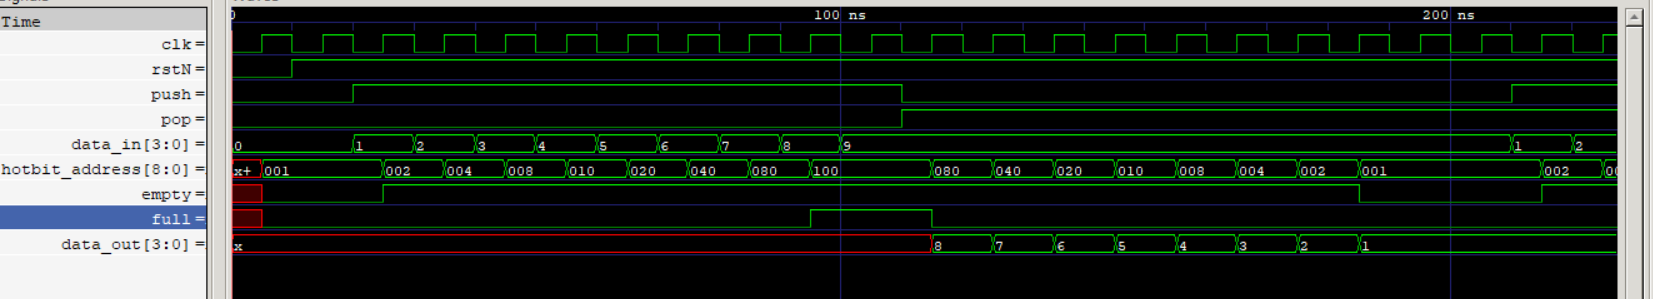
\includegraphics[width = 0.9\textwidth]{graphics/waveform.png}
	\end{figure}
\end{document}